% -*- mode: LaTeX; TeX-PDF-mode: t; -*- 
% LaTeX path to the root directory of the current project
% from the directory in which this file resides
% and path to econtexPaths which defines the rest of the paths like \FigDir
\providecommand{\econtexRoot}{}\renewcommand{\econtexRoot}{.}
\providecommand{\econtexPaths}{}\renewcommand{\econtexPaths}{econtexPaths}
% -*- mode: LaTeX; TeX-PDF-mode: t; -*- 
% The \commands below are required to allow sharing of the same base code via Github between TeXLive on a local machine and Overleaf (which is a proxy for "a standard distribution of LaTeX").  This is an ugly solution to the requirement that custom LaTeX packages be accessible, and that Overleaf prohibits symbolic links
\providecommand{\packages}{\econtexRoot/Resources/texmf-local/tex/latex}
\providecommand{\econtex}{\packages/econtex}
\providecommand{\econark}{\econtexRoot/Resources/texmf-local/tex/latex/econark}
\providecommand{\econtexSetup}{\econtexRoot/Resources/texmf-local/tex/latex/econtexSetup}
\providecommand{\econarkSetup}{\econtexRoot/Resources/texmf-local/tex/latex/econarkSetup}
\providecommand{\econtexShortcuts}{\econtexRoot/Resources/texmf-local/tex/latex/econtexShortcuts}
\providecommand{\econtexBibMake}{\econtexRoot/Resources/texmf-local/tex/latex/econtexBibMake}
\providecommand{\econtexBibStyle}{\econtexRoot/Resources/texmf-local/bibtex/bst/econtex}
\providecommand{\econtexBib}{economics}
\providecommand{\notes}{\econtexRoot/Resources/texmf-local/tex/latex/handout}
\providecommand{\handoutSetup}{\econtexRoot/Resources/texmf-local/tex/latex/handoutSetup}
\providecommand{\handoutShortcuts}{\econtexRoot/Resources/texmf-local/tex/latex/handoutShortcuts}
\providecommand{\handoutBibMake}{\econtexRoot/Resources/texmf-local/tex/latex/handoutBibMake}
\providecommand{\handoutBibStyle}{\econtexRoot/Resources/texmf-local/bibtex/bst/handout}

\providecommand{\FigDir}{\econtexRoot/Figures}
\providecommand{\CodeDir}{\econtexRoot/Code}
\providecommand{\DataDir}{\econtexRoot/Data}
\providecommand{\SlideDir}{\econtexRoot/Slides}
\providecommand{\TableDir}{\econtexRoot/Tables}
\providecommand{\ApndxDir}{\econtexRoot/Appendices}

\providecommand{\ResourcesDir}{\econtexRoot/Resources}
\providecommand{\rootFromOut}{..} % APFach back to root directory from output-directory
\providecommand{\LaTeXGenerated}{\econtexRoot/LaTeX} % Put generated files in subdirectory
\providecommand{\econtexPaths}{\econtexRoot/Resources/econtexPaths}
\providecommand{\LaTeXInputs}{\econtexRoot/Resources/LaTeXInputs}
\providecommand{\LtxDir}{LaTeX/}
\providecommand{\EqDir}{\econtexRoot/Equations} % Put generated files in subdirectory

\providecommand{\titlepagecustom}{\LaTeXInputs/titlepagecustom}


\documentclass[\econtexRoot/HAFiscal]{subfiles}
\onlyinsubfile{\providecommand{\econtexRoot}}
\onlyinsubfile{\renewcommand{\econtexRoot}{..}}
\onlyinsubfile{\externaldocument{\econtexRoot/HAFiscal}} % Get xrefs -- esp to apndx -- from main file; only works if main file has already been compiled

\begin{document}

\FloatBarrier
\hypertarget{comparing-fiscal-stimulus-policies}{}\par\section{Comparing fiscal stimulus policies}
\notinsubfile{\label{sec:comparing}}

In this section, we present our results where we compare three policies to provide fiscal stimulus in our calibrated model. The policies we compare are a means-tested stimulus check, an extension of unemployment benefits, and a payroll tax cut. Each policy is implemented at the start of a recession, and we compare results both with and without aggregate demand effects being active during the recession. First, we present impulse responses of aggregate income and consumption after the implementation of each policy. Then we compare the policies in terms of their cumulative multipliers and in terms of their effect on a welfare measure that we introduce. Finally, based on these comparisons, we can rank the three policies. 

\hypertarget{impulse-responses}{}\par\subsection{Impulse responses}
\notinsubfile{\label{sec:IRFs}}

The impulse responses that we present for each stimulus policy are constructed as follows: 
\begin{itemize} 
\item A recession hits in quarter one. 
\item We compute the subsequent path for the economy without any policy introduced in response to the recession. 
\item We also compute the subsequent path for the economy with a given policy introduced at the onset of the recession in quarter one. 
\item The impulse responses we present are then the \textit{difference} between these two paths for the economy and show the effect of a policy relative to a case where no policy was implemented.
\item The solid lines show these impulse responses for an economy where the aggregate demand effects described in section~\ref{sec:ADeffects} are not active, and the dashed lines show impulse responses for an economy where the aggregate demand effects are active during the recession. 
\item Red lines refer to aggregate labor and transfer income, and blue lines refer to consumption. 
\end{itemize}

Note that all graphs show the average response of income and consumption for recessions of different length.
Specifically, we simulate recessions lasting from only one quarter up to 20 quarters.
We then take the sum of the results across all recession lengths weighted by the probability of this recession length occurring (given our assumption of an average recession length of six quarters).

\subsubsection{Stimulus check} 

\begin{figure}
  \centering
  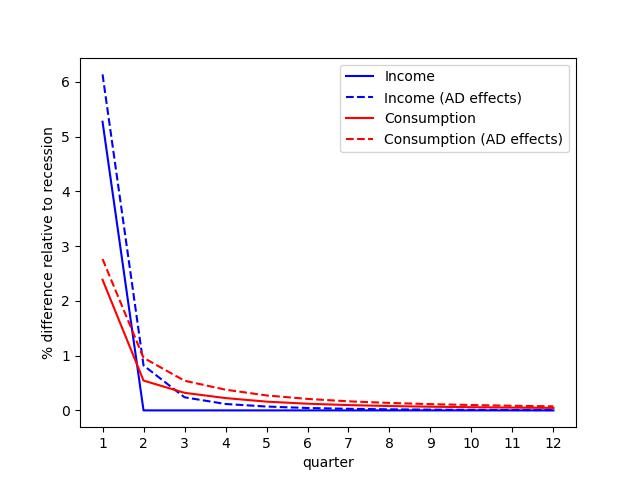
\includegraphics[width=0.8\linewidth]{\econtexRoot/Code/HA-Models/FromPandemicCode/Figures/recession_Check_relrecession}
  \caption{Impulse responses of aggregate income and consumption to a \textbf{stimulus check} during recessions with and without aggregate demand effects}
  \notinsubfile{\label{fig:recessioncheckrelrecession}}
\end{figure}

Figure \ref{fig:recessioncheckrelrecession} shows the impulse response of income and consumption when stimulus checks are issued in the first quarter of a recession.
In the model without a multiplier, the stimulus checks account for 5.5 percent of the first quarter's income.
In the following quarters, there are no further stimulus payments, and income remains the same as it would have been without the stimulus check policy.
Consumption is about 3 percent higher in the first quarter, which includes the splurge response to the stimulus check.
Consumption then drops to less than 1 percent above the counterfactual, and the remainder of the stimulus check money is then spent over the next few years.
In the model with aggregate demand effects, income in the first quarter is 6.5 percent higher than the counterfactual, as the extra spending feeds into higher incomes.
Consumption in this model jumps to a higher level than without aggregate demand effects and comes down more slowly as the feedback effects from consumption to income damp the speed with which income---and hence the splurge---return to zero.
After a couple of years, when the recession is most likely over and aggregate demand effects are no longer in place, income is close to where it would be without the stimulus check policy, although consumption remains somewhat elevated.

\subsubsection{UI extension}

\begin{figure}
  \centering
  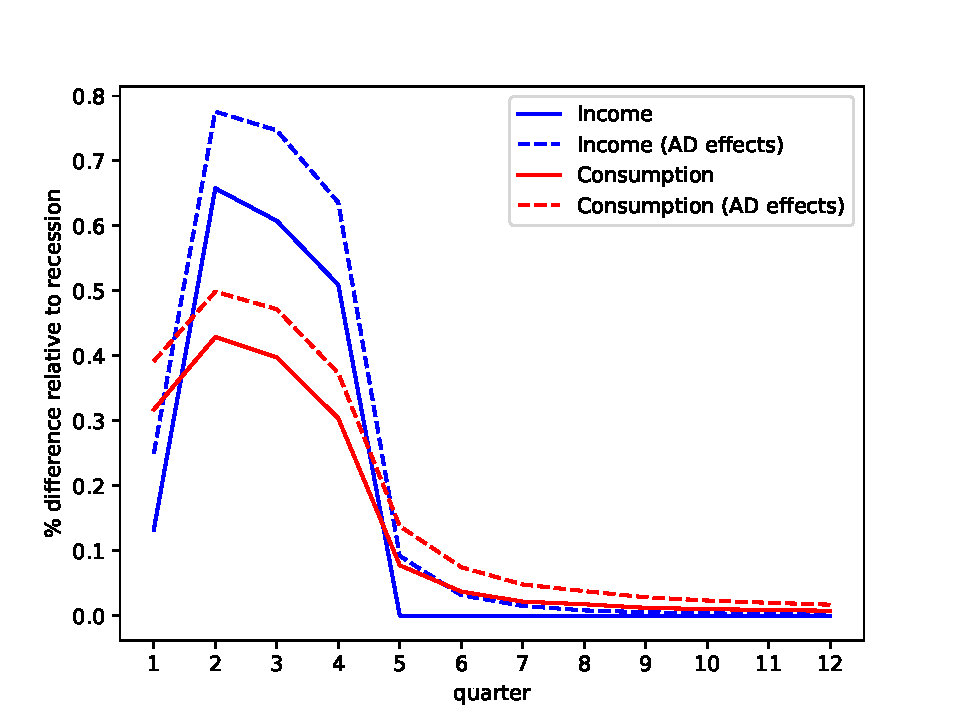
\includegraphics[width=0.8\linewidth]{Code/HA-Models/FromPandemicCode/Figures/recession_UI_relrecession}
  \caption{Impulse responses of aggregate income and consumption to a \textbf{UI extension} during recessions with and without aggregate demand effects}
  \notinsubfile{\label{fig:recessionuirelrecession}}
\end{figure}

The impulse responses in figure \ref{fig:recessionuirelrecession} show the response to a policy that extends unemployment benefits from 6 months to 12 months for a period of a year.
In the model without aggregate demand effects, the path for income now depends on the number of consumers who receive the extended unemployment benefits.
These consumers are those who have been unemployed for between 6 and 12 months.
In the first quarter of the recession, the newly unemployed receive unemployment benefits regardless of whether they are extended or not.
Therefore, it is in the second and third quarters, when the effects of the recession on long-term unemployment start to materialize, that the extended UI payments ramp up, amounting to an aggregate increase in quarterly income by 0.7 percent.
By the fifth quarter, the policy is no longer in effect, and income from extended unemployment goes to zero.
Consumption in the first quarter jumps by more than income (by 0.3 percent), prompted by both the increase in expected income and the reduced need for precautionary saving given the extended insurance.
In the model without aggregate demand effects, consumption is only a little above the counterfactual by the time the policy is over.
In the model with aggregate demand effects, there is an extra boost to income of about the same size in the first and second quarters.
As this extra aggregate demand induced income goes to employed consumers, more of it is saved, and consumption remains elevated several quarters beyond the end of the policy.

\subsubsection{Payroll tax cut}

\begin{figure}
  \centering
  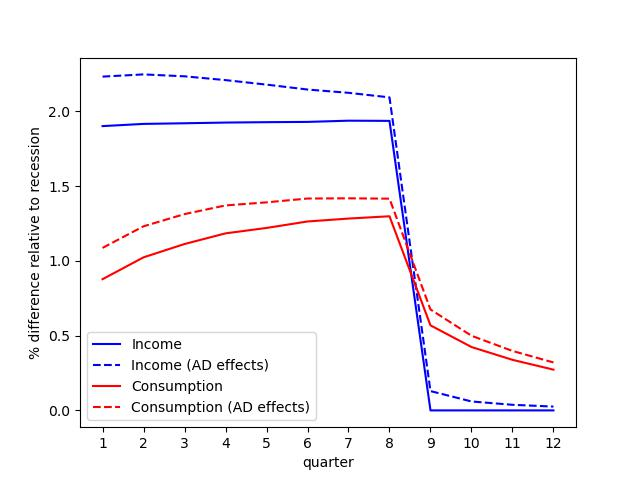
\includegraphics[width=0.8\linewidth]{Code/HA-Models/FromPandemicCode/Figures/recession_taxcut_relrecession}
  \caption{Impulse responses of aggregate income and consumption to a \textbf{payroll tax cut} lasting eight quarters during recessions with and without aggregate demand effects}
  \notinsubfile{\label{fig:recessiontaxcutrelrecession}}
\end{figure}

The final impulse response graph, figure \ref{fig:recessiontaxcutrelrecession}, shows the impulse response for a payroll tax cut that persists for two years (eight quarters).
In the model without aggregate demand effects, income rises by close to 2 percent as the take-home pay for employed consumers goes up.
After the two-year period, income drops back to where it would have been without the payroll tax cut.
Consumption jumps close to 1.3 percent in response to the tax cut.
Over the period in which the tax cut is in effect, consumption rises somewhat as the stock of precautionary savings goes up, before declining in anticipation of the drop in income at the two-year mark.
Following the drop in income, consumption drops sharply because of the splurge and then decreases over time as consumers spend out the savings they built up over the period the tax cut was in effect.
In the model with aggregate demand effects, income rises by about 2.5 percent above the counterfactual and then declines steadily as the probability that the recession remains active---and hence the aggregate demand effects in place---goes down over time.\footnote{Again, consumption tends to first rise because of the build-up of precautionary savings, before falling again as the probability that the recession remains in place declines.
This hump-shaped pattern feeds through to income, explaining the upward trend in income during the first two quarters.} In response to the now declining expected path for income over the two years during which the tax cut remains in place, consumption also declines, albeit at a slightly slower pace.
Following the end of the policy, the savings stock in the model with aggregate demand effects is high, and consumption remains significantly elevated through the period shown.

\hypertarget{multipliers}{}\par\subsection{Multipliers}
\notinsubfile{\label{sec:multipliers}}

In this section, we compare the fiscal multipliers across the three stimulus policies.
Specifically, we employ the cumulative multiplier, which captures the ratio between the net present value (NPV) of stimulated consumption up to horizon $t$ and the full-horizon NPV of the cost of the policy.
We thus define the cumulative multiplier up to horizon $t$ as
\begin{equation*}
  M(t) = \frac{NPV(t,\Delta C)}{NPV (\infty,\Delta G)},
\end{equation*}
where $\Delta C$ is the additional aggregate consumption spending up to time $t$ in the policy scenario relative to the baseline and $\Delta G$ is the total government expenditure caused by the policy.
The NPV of a variable $X_t$ is given by 
$NPV(t,X) = \sum_{s=0}^{t} \left( \prod_{i=1}^{s} \frac{1}{R_i} \right) X_s$.


\begin{figure}[t]
  \centering
  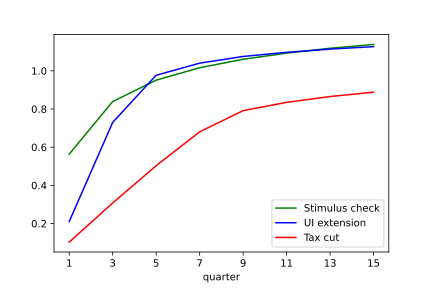
\includegraphics[width=0.8\linewidth]{Code/HA-Models/FromPandemicCode/Figures/Cummulative_multipliers}
  \caption{Cumulative multiplier as a function of the horizon for the three policies. Note: Policies are implemented during a recession with AD effect active.}
  \notinsubfile{\label{fig:cumulativemultipliers}}
\end{figure}

Figure \ref{fig:cumulativemultipliers} plots the cumulative multipliers at different horizons, and table~\ref{tab:Multiplier} shows the 10y-horizon multiplier for each policy.
The stimulus check, which is paid out in quarter one, exhibits the largest multiplier on impact.
About 60 percent of the total policy expenditure is immediately spent by consumers.
After one year, and because of the aggregate demand effects, consumption has increased cumulatively by more than the cost of the stimulus check.
Over time, the policy reaches a total multiplier of 1.245.
Without AD effects the policy only generates a multiplier of 0.872.

The multiplier is slightly lower for the UI extension policy than the stimulus check over most horizons.
Since spending for the UI policy is spread out over four quarters (and peaks in quarters two to three), the multiplier in the first quarter is considerably lower than in the case of the stimulus check.
The UI extension policy is targeted in the sense that it provides additional income to only those consumers, who, because of unemployment, have large MPCs.
However, it is slow to roll out, and some of the spending occurs at later quarters, when the recession might have ended.
Overall, around 80 percent of the policy expenditure occurs during the recession.
In contrast, the stimulus check is paid out fully during the first quarter, when, by construction, the recession occurs with certainty.
Therefore, the aggregate demand effects are particularly potent for the stimulus check policy despite being less targeted and providing stimulus also to agents with low MPCs relative to the extended UI policy.

\begin{table}[t]
  \center
  \begin{tabular}{@{}lccc@{}} 
\toprule 
& Tax Cut    & UI extension    & Stimulus check    \\  \midrule 
Long-run Multiplier (AD effect) &0.968  & 1.180  & 1.228     \\ 
Long-run Multiplier (1st round AD effect only) &0.000  & 0.000  & 0.000     \\ 
Share of policy expenditure during recession &45.0\%  & 72.0\%  & 100.0 \%    \\ 
\end{tabular}  

  \caption{Multipliers as well as the share of the policy occurring during the recession}
  \notinsubfile{\label{tab:Multiplier}}
\end{table}

The payroll tax cut has the lowest multiplier irrespective of the considered horizon.
A multiplier of 1 is reached only after 10 years with AD effects.
These relatively small numbers reflect that policy spending lasts for a long time and is thus more likely to occur after the recession has ended.
Moreover, only employed consumers, often with relatively low MPCs, benefit directly from the payroll tax cut.
Therefore, the policy is poorly targeted if the goal is to provide short-term stimulus.

Table \ref{tab:Multiplier} contains an additional (middle) row.
To understand these values note that the policies initially increase the income of consumers directly, which leads to a boost in consumption.
As a consequence, this boost triggers an aggregate demand effect which increases the income of everyone and in turn leads to an additional boost to consumption.
We refer to the sum of this initial and the indirect boost to consumption as the first-round AD effect.
However, the AD effect continues as the indirect boost to consumption triggers another round of income increases which further boost consumption and so on.
One might argue that these higher-order rounds of the AD effect are not likely to be anticipated by consumers.
Since higher-order consumption boosts only materialize if consumers anticipate them and act accordingly, the overall increase in consumption might turn out to be smaller than suggested by the full AD effect.
The middle row of the table shows the multipliers that result in the special case where we only consider the first-round AD effect.
As expected, the multipliers are smaller when excluding higher-order rounds.
Nevertheless, the ranking of the policies remain unchanged.

\hypertarget{welfare}{}\par\subsection{Welfare}
\notinsubfile{\label{sec:welfare}}

In this section, we look at the welfare implications of each stimulus policy.
To do so, we need a way to aggregate welfare in our model with individual utility functions.
Our approach to constructing a welfare measure is based on three principles:
\begin{enumerate}
\item The felicity of each consumer at any moment in time is valued equally by the social planner.  However, the planner has a personal discount rate, which may not coincide with that of any consumer in the model.
\item There is no social benefit or cost to implementing any of the policies outside of a recession. 
\item Utility is gained from splurge spending in the same way as other spending.
\end{enumerate} 

The first of these principles would suggest that a simple aggregation of consumers' utilities, discounted at the social planner's discount rate, is appropriate.
However, this simple aggregation would give the social planner a large incentive to redistribute income from high- to low-consumption households, even during normal times, which runs against the second principle.
Instead, we use the aggregated utility function as a building block.
Let  $\mathcal{W}(\text{policy},Rec,AD)$ be the aggregated utility function:
\begin{equation}\begin{gathered}\begin{aligned}
  \mathcal{W}(\text{policy},Rec,AD) =\frac{1}{N}\sum_{i=1}^{N} \sum_{t=0}^{\infty} \beta_S^t u(\mathbf{c}_{it,\text{policy},Rec,AD}) ,
\end{aligned}\end{gathered}\end{equation}
where $\text{policy}\in \{\text{None, Stimulus Check, UI extension, Payroll Tax Cut}\}$ is the stimulus policy followed, $Rec\in\{1,0\}$ is an indicator for whether the policy coincides with the start of a recession or is implemented in nonrecessionary times, and $AD\in\{1,0\}$ is an indicator for whether the aggregate demand effects are active during the recession.
$\mathbf{c}_{it,\text{policy},Rec,AD}$ are the consumption paths (including the splurge) for each consumer $i$ in each scenario.
$\beta_S$ is the social planner's discount factor that we will set equal to the inverse of the real interest rate $R$.
$N$ is the number of consumers simulated.

We use the steady-state baseline as a way to convert from welfare units to consumption units.
Using this baseline, we define the marginal increase in welfare that occurs when every consumer increases consumption proportionally to baseline consumption as the following\footnote{Note that with log utility, $\mathcal{W}^c =\frac{1}{N}\sum_{i=1}^{N} \sum_{t=0}^{\infty} \beta_S^t = \frac{1}{1-\beta_S}$}
\begin{equation}\begin{gathered}\begin{aligned}
  \mathcal{W}^c =\frac{1}{N}\sum_{i=1}^{N} \sum_{t=0}^{\infty} \beta_S^t \mathbf{c}_{it,\text{None},0,0} u'(\mathbf{c}_{it,\text{None},0,0}) .
\end{aligned}\end{gathered}\end{equation}
With this definition, we consider, in steady-state consumption units $\mathcal{W}^c$, the increase in welfare induced by a policy: $\frac{\mathcal{W}(\text{policy},Rec,AD)-\mathcal{W}(\text{None},Rec,AD)}{\mathcal{W}^c}$.
However, this welfare increase ignores the cost of the policy to the government, $PV(\text{policy},Rec)$.\footnote{For the stimulus check and extended UI, the payments made by the government are clearly defined and do not depend on aggregate demand effects.
For the payroll tax cut, we define the payments as the difference between the take-home pay with and without the tax cut, but ignoring any aggregate demand effects.
Aggregate demand effects would increase the value of the tax cut because incomes would rise, but, in fact, the effects increase rather than decrease the tax receipts of the government.} We therefore subtract the fiscal cost of each policy in steady-state consumption units:  $\frac{PV(\text{policy},Rec)}{{P}^c}$, where ${P}^c$, the marginal cost of increasing every consumer's steady-state consumption proportionally, is given by
\begin{equation}\begin{gathered}\begin{aligned}
  \mathcal{P}^c = \frac{1}{N}\sum_{i=1}^{N} \sum_{t=0}^{\infty} R^{-t} \mathbf{c}_{it,\text{None},0,0} .
\end{aligned}\end{gathered}\end{equation}
Finally, we normalize the welfare benefit by subtracting the welfare effect of the policy in non-recessionary times.
This normalization can be thought to encompass both the preferences of society not to redistribute and the negative incentive effects of redistribution in normal times.
Our final welfare measure, expressed in units of steady-state consumption, is
\begin{equation}\begin{gathered}\begin{aligned}
  \mathcal{C}(\text{policy},Rec,AD) &= \bigg(\frac{\mathcal{W}(\text{policy},Rec,AD)-\mathcal{W}(\text{None},Rec,AD)}{\mathcal{W}^c} - \frac{PV(\text{policy},Rec)}{\mathcal{P}^c} \bigg) \nonumber \\  
                                    & \qquad -
                                      \bigg(\frac{\mathcal{W}(\text{policy},0,0) - \mathcal{W}(\text{None},0,0)}{\mathcal{W}^c} - \frac{PV(\text{policy},0)}{\mathcal{P}^c} \bigg) \notinsubfile{\label{welfare_defn}}.
\end{aligned}\end{gathered}\end{equation}

Table \ref{welfare} shows the welfare benefits of each policy as defined by equation \eqref{welfare_defn}.
The stimulus check and payroll tax cut policies have been adjusted to be the same fiscal size (in the absence of a recession) as the UI extension.\footnote{Specifically, we reduce the size of the stimulus check from \$1200 to \$80 per person, while the payroll tax cut is reduced from a 2 pp to a 0.05 pp cut.
We have verified that the multiplier for check stimulus and the tax cut is only marginally changed by the downscaling.} The table shows consumption-equivalent welfare gains in basis points, which are to be interpreted as follows.
A welfare gain of $x$ implies that the social planner is indifferent between the stimulus policy being implemented in response to a recession and a permanent increase in the baseline consumption of the total population by $x$ basis points (that is a one-hundredth of~1 percent of the baseline consumption).
We will, however, first discuss the relative differences across the policies and then discuss the magnitude of the welfare effects.

Without aggregate demand effects (the first row of the table), the payroll tax cut has extremely limited welfare benefits compared with the other policies.
The reason is that the payroll tax cut goes to consumers who remain employed, and therefore it does not directly affect the unemployed consumers who are the most hit by the recession.
However, employed consumers do reduce their consumption at the onset of the recession because of the increased unemployment risk, so the tax cut helps them more than in nonrecessionary times.
Similarly, the stimulus check has limited benefits relative to the UI policy, as it mostly goes to employed consumers, although it has the benefit over the payroll tax cut of also reaching those made unemployed and those who remain unemployed because of the recession.
The extended UI policy is the clear ``bang for the buck'' winner, as the extended UI payments are well targeted to the households who are particularly severely hit by the recession, giving rise to large welfare improvements relative to pursuing the policy in normal times.

The second row of the table shows the welfare benefits in the version of the model with aggregate demand effects during the recession.
The payroll tax cut now has a noticeable benefit, as some of the tax cut gets spent during the recession, resulting in higher incomes for all consumers.
However, the tax cut is received over a period of two years, and much of the relief may be after the recession---and hence the aggregate demand effect---is over.
Furthermore, because the payroll tax cut goes only to employed consumers who have relatively lower MPCs, the spending out of this stimulus will be further delayed, possibly beyond the period of the recession.
By contrast, the stimulus check is received in the first period of the recession and goes to both employed and unemployed consumers.
The earlier arrival and higher MPCs of the stimulus check recipients mean more of the stimulus is spent during the recession, leading to greater aggregate demand effects, higher income, and higher welfare.
The extended UI arrives, on average, slightly later than the stimulus check.
However, the recipients, who have been unemployed for at least six months, spend the extra benefits relatively quickly, resulting in significant aggregate demand effects during the recession.
In contrast to the payroll tax cut, extended UI has the benefit of automatically reducing if the recession ends early, making fewer consumers eligible for the benefit.

The welfare effects for the UI extension are largest compared with other stimulus policies when those policies are scaled down to match the total expenditure size of the UI extension policy.
Nevertheless, the welfare effect of the UI extension is relatively modest, amounting to only 1.101 basis points of baseline consumption.
However, while the UI extension policy cannot be easily scaled to a larger size, scaling is certainly possible for the stimulus check.
If we consider a \$1,200 stimulus check rather than the \$80 check underlying the calculations in table \ref{welfare}, we obtain---using a simple back-of-the-envelope calculation---a welfare gain equivalent to 0.151 $\times \frac{1200}{80} = $ 2.3 basis points of baseline consumption.
If we then assume that the average consumer experiences recessions five times during a lifetime, the welfare gain of this policy being implemented during recessions is $2.3\times 5 $ = 11.5 basis points, which is larger than the welfare cost estimated in \cite{Lucas1987models} for business cycle fluctuations.

\begin{table}[ht] 
  \center
  \begin{tabular}{@{}lccc@{}} 
\toprule 
                          & Check      & UI    & Tax Cut    \\  \midrule 
$\mathcal{C}(Rec,\text{policy})$ & 0.737  & 1.845  & 0.156     \\ 
$\mathcal{C}(Rec, AD,\text{policy})$ & 3.049  & 2.514  & 2.711     \\ 
\end{tabular}  

  \caption{Consumption-equivalent welfare gains in basis points, calculated for policies implemented in a recession with and without aggregate demand effects}
  \notinsubfile{\label{welfare}}
\end{table}

\hypertarget{comparing-the-policies}{}\par\subsection{Comparing the policies} 

The results presented in sections~\ref{sec:multipliers} and~\ref{sec:welfare} indicate that the extension of unemployment benefits is the clear ``bang for the buck'' winner.
The extended UI payments are well targeted to consumers with high MPCs and high marginal utility, giving rise to large multipliers and welfare improvements.
The stimulus checks come in slightly higher when measured by their multiplier effect but are a distant second when measured by their welfare effects.
The stimulus checks have large multipliers because the money gets to consumers at the beginning of the recession and is therefore most likely to be spent during the recession when spending passes through to productivity.
However, the checks are not well targeted to high-MPC consumers, so even though the funds arrive early in the recession, they are spent out more slowly than the extended unemployment benefits.\footnote{Theoretically, stimulus checks could be targeted to the highest-MPC households which, for small-sized policies, would mean households with an MPC of one.
However, data limitations and other practicalities make means-testing stimulus checks by income the extent of targeting in practice.} Furthermore, the average recipient of a stimulus check has a much lower marginal utility than consumers receiving unemployment benefits, so the welfare benefits of this policy are substantially muted relative to UI extensions.

The payroll tax cut policy does poorly by both measures: It has a low overall multiplier and negligible welfare benefits.
The reasons are that the funds are slow to arrive, so the subsequent spending often occurs after the end of the recession, and that the payments are particularly badly targeted---they go only to employed consumers.

While it is clear from the analysis that the extended unemployment benefits should be the first tool to use, a disadvantage of them is that they are limited in their size.
If a larger fiscal stimulus is deemed appropriate, then stimulus checks provide an alternative option that will stimulate spending during the recession even if the welfare benefits are substantially lower than the UI extension.

\ifthenelse{\boolean{Web}}{}{
  \end{document} \endinput
}
